\paragraph{АР-модель}

В третьей главе рассматривается параметрический метод оценки частоты на основе авторегрессионной (АР) - модели сигнала.
АР модель ${P}$-го порядка может быть представлена следующим образом \cite{marpl_book, saeed_book}:

\begin{equation}
	\label{eq:ar_model}
	y(m) = \sum \limits_{k=1}^{P} a_k y(m-k) + n(m)
\end{equation}
где ${a_k}$ - коэффициенты АР-модели, $n(t)$ - шумовая компонента.

\begin{figure}[H]
	\center\scalebox{1}{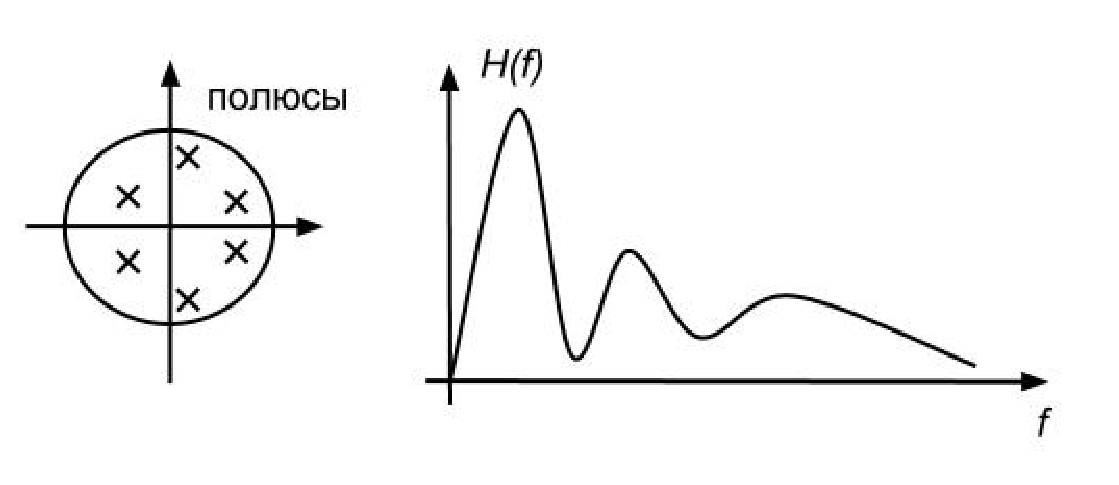
\includegraphics[width=1\linewidth]{lpc_poles.eps}}
	\caption{Полюса и АЧХ линейного предсказателя}
	\label{pic:ar_poles}
\end{figure}

На рисунке \ref{pic:ar_poles} изображен пример расположения полюсов и соответствующие им пики частотной характеристики АР модели \ref{eq:ar_model}.
Для действительного сигнала каждая пара комплексно сопряженных полюсов определяет положение и форму одного частотного пика характеристики.

ля обнаружения гармонического сигнала одной частоты на фоне аддитивной помехи в виде белого шума достаточно использовать АР модель второго порядка.
В этом случае оценка параметров модели методом наименьших квадратов (МНК) может быть записана в матричном виде:

\begin{center}
\begin{equation}
	\label{eq:ar_coef_matrix}
	\left[ \begin{array}{c}
		\hat{a}_1 \\
		\hat{a}_2
	\end{array} \right]
	=
		\left[ \begin{array}{cc}
			r_{xx}(0)  + \sigma_n^2 & r_{xx}(1)\\
			r_{xx}^*(1) & r_{xx}(0) + \sigma_n^2 
		\end{array} \right]^{-1}
		\left[ \begin{array}{c}
			r_{xx}(1) \\
			r_{xx}(2)
		\end{array} \right]
	= R_x^{-1}r_{xx1}
\end{equation}
\end{center}
здесь ${\hat{a}_1, \hat{a}_2}$ - МНК оценки коэффициентов АР-модели, ${r_{xx}(m)}$ - автокорреляционная функция (АКФ) принимаемого сигнала,
${\sigma_n^2}$ - дисперсия белого шума.  Для оценки АКФ ${\hat{r}_{xx}}$ можно использовать выражение:

\begin{equation}
	\label{eq:af_acf_est}
	r_{xx}(m) = \frac{1}{N-1}\sum \limits_{k=0}^{N-1}x(k)x(k-m)
\end{equation}

При этом для учета шума следует скорректировать полученную оценку следующим образом: ${\hat{r}_{xx}(0) = r_{xx}(0) - \sigma_n^2}$.
Предполагается, что мощность теплового шума известна и одинакова для всех источников сигнала. 

Передаточная функция АР модели второго порядка ${H(z)}$:
\begin{equation}
	\label{eq:af_transfer_func}
	H(z) = \frac{1}{1 - a_1 z^{-1} - a_2 z^{-2}}
\end{equation}

Для определения резонансной частоты ${H(z)}$ можно воспользоваться формулой:
\begin{equation}
	\label{eq:af_omega}
	\omega_0 = arg(z_1)
\end{equation}
где ${z_{1,2} = re^{(\pm j \omega_0)}}$ - полюса передаточной функции \ref{eq:af_transfer_func}. Для принятия решения о наличии гармонического сигнала
анализируют значение квадрата модуля частотной характеристики АР-модели в точке резонанса:

\begin{equation}
	\label{eq:af_transfer_func}
	\left| H(\omega_0) \right| ^2 = \frac{1}{ \left| 1 - a_1 e^{-j \omega_0} - a_2 e^{-j2 \omega_0} \right| ^2}
\end{equation}

Если это значение превышает некоторый заранее выбранный порог, то принимается решение о наличии гармонического сигнала с частотой ${\omega_0}$.
Полюсы и частотный ответ для АР модели второго порядка представлены на рисунке \ref{pic:ar_poles_afc}. На рисунке штриховым обозначен
спектр входного сигнала, а сплошным спектр входного сигнала после демодуляции ПСП.

\begin{figure}[H]
	\center\scalebox{1}{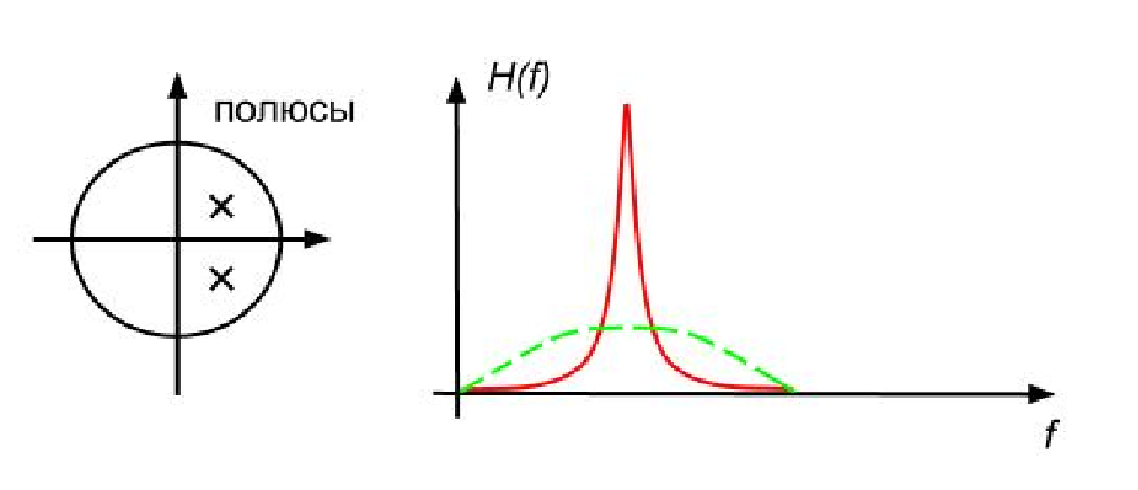
\includegraphics[width=1\linewidth]{lpc_poles_gps.eps}}
	\caption{Полюс и АЧХ ФР-модели второго порядка}
	\label{pic:ar_poles_afc}
\end{figure}

Удобство применения АР для задачи оценки частоты обусловлено тем, что в сигнале с расширенным спектром после демодуляции ПСП остается одна
гармоническая компонента и шум – выражение \ref{eq:cdma_strip_eq}.  Даже если входной сигнал содержал другие гармонические компоненты,
после повторной модуляции они будут "размазаны" по спектру.
